\documentclass[11pt]{article}

\usepackage[letterpaper,bindingoffset=0.2in,
            left=1in,right=1in,top=0.75in,bottom=1in,
            footskip=.25in]{geometry}

\usepackage{hyperref}
	\hypersetup{
			colorlinks=true,
			linkcolor=black,
			filecolor=magenta,      
			urlcolor=blue,
	}
	
\usepackage{graphicx}
	\graphicspath{ {images/} }
	
\usepackage{subcaption}
	
\begin{document}


\title{COMP SCI 5401 FS2017 Assignment 2a}
\author{Stuart Miller\\\href{mailto:sm67c@mst.edu}{sm67c@mst.edu}}
\maketitle


\section{Overview}\label{sect:overview}

Assignment 2a provides an introduction to the Iterative Prisoner's Dilemma problem by implementing a random search. 


\section{Algorithm Strategy}\label{sect:alg_strat}
The algorithm works by generating a random tree than playing it tit-for-tat for a set number of iterations. This means that its opponent will choose whatever option the agent chose last round for itself.


\section{Analysis}\label{sect:analysis}
The agents tend to converge pretty quickly on one particular strategy. As you can see in Figure \ref{fig:default}, the agent's fitness doesn't change at all after the first few iterations. Zooming in as shown in Figure \ref{fig:default_limited} illustrates this convergence. Some runs immediately reach a value, others approach it steadily. Most agents end up close to the 3 fitness mark. This makes sense because the most valuable choice for both agents is to mutually confess. Only once did it manage to find a solution where it could converge on a payoff of 5 by exploiting the opponent.

\begin{figure}[h]
\begin{minipage}{.5\textwidth}
  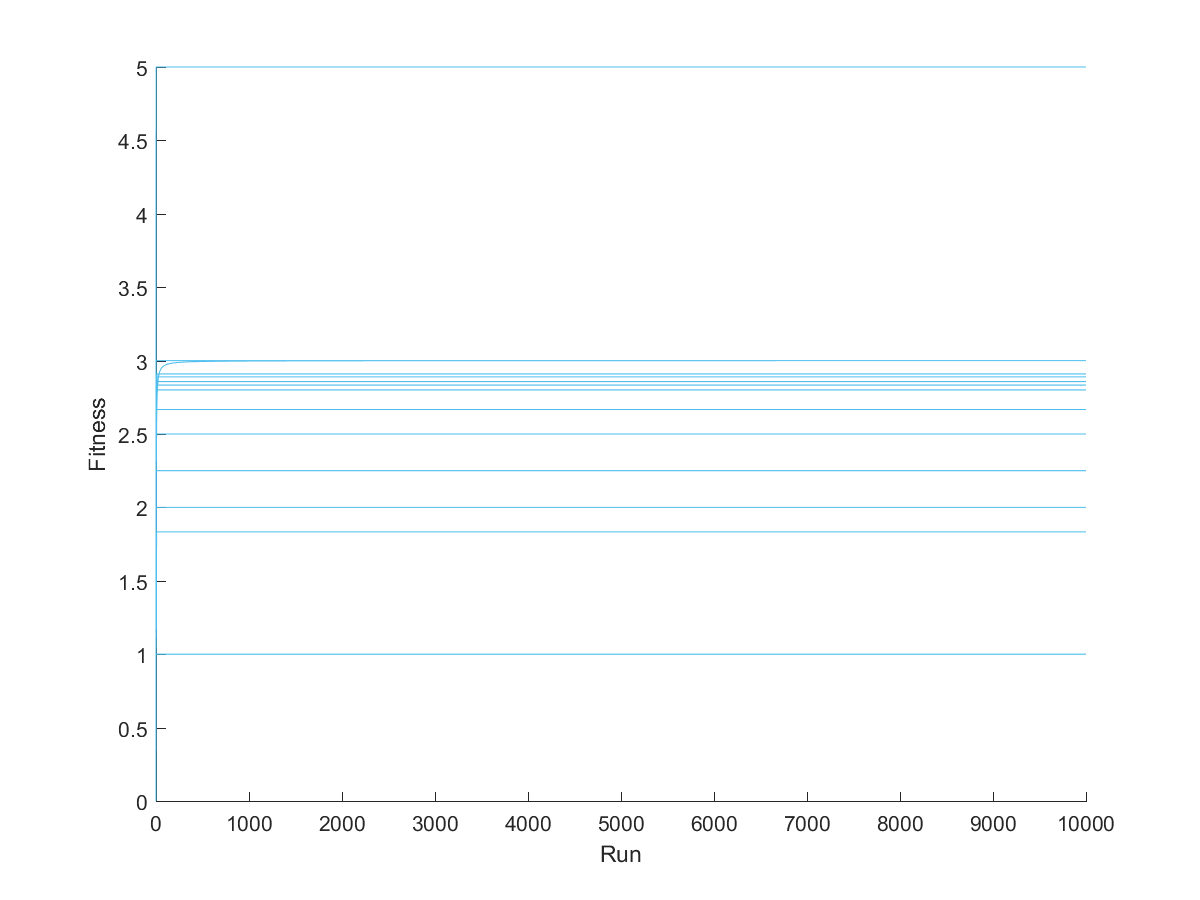
\includegraphics[width=3.25in]{default.png}
  \captionof{figure}{\\Fitness vs. Evals plot}
  \label{fig:default}
\end{minipage}%
\begin{minipage}{.5\textwidth}
  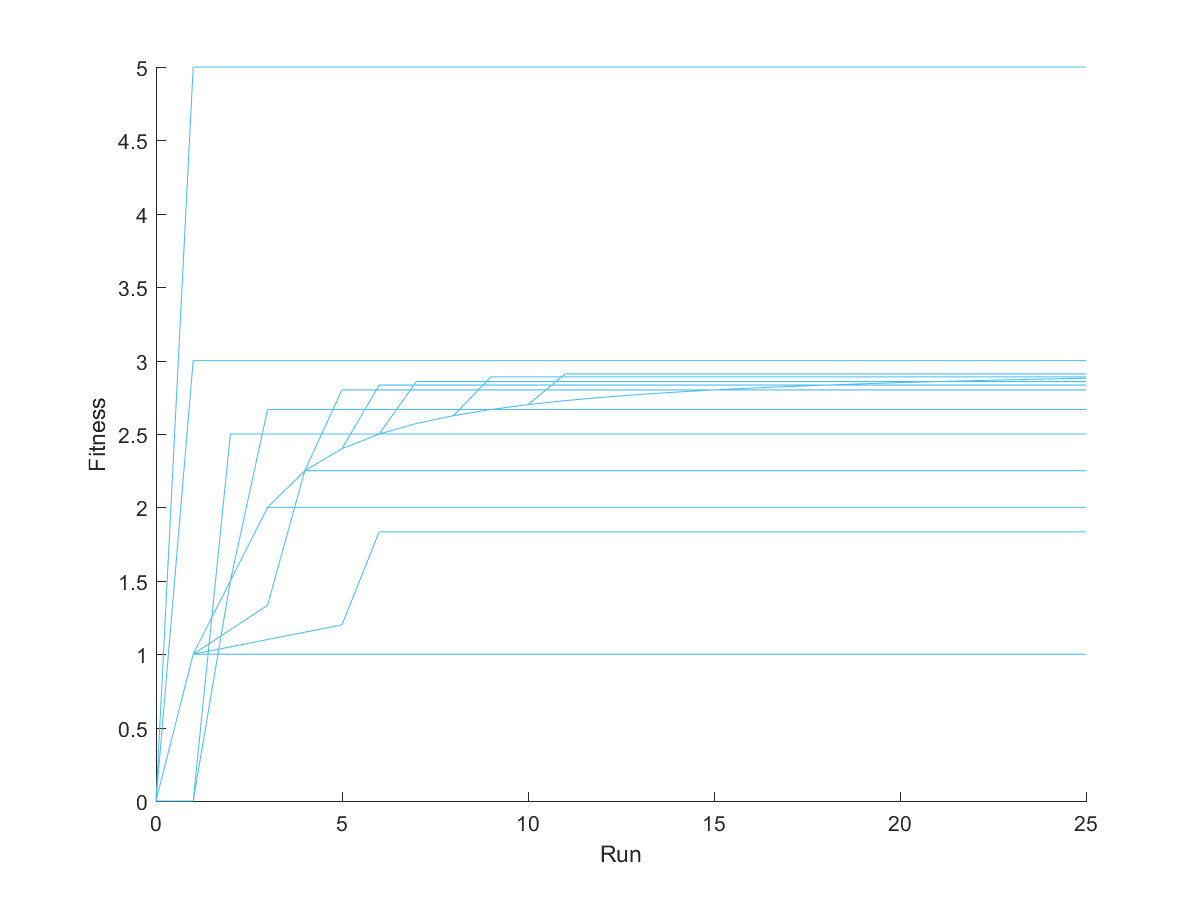
\includegraphics[width=3.25in]{default_limited.png}
  \captionof{figure}{\\Fitness vs. Evals plot\\Limited to 0,25 }
  \label{fig:default_limited}
\end{minipage}
\end{figure}

\end{document}